% Preamble
\documentclass[11pt]{article}

% Packages
\usepackage{amsmath}
\usepackage{graphicx}

% Title and Author
\title{Situationally Aware Mesa Optimisers will have Long Term Objectives}
\author{Andreas Moe}
\date{\today}

% Document
\begin{document}

\maketitle

\section*{Abstract}

\section{Backround}\label{sec:backround}

Hubinger et al.\cite{hubinger2021} introduced the concept of a mesa optimiser, an optimiser being optimised by
an optimiser.
They conjecture that a mesa optimiser can arise naturally in a machine learning context, where the outer optimiser is
the machine learning algorithm.
This raises a safety issue, known as goal misgeneralisation.
This issue, studied by Jack Koch et al. \cite{jackkoch2023}, arises when a mesa optimiser has learned a goal
(mesa objective), which correlates with the RL rewards (base objective) on the training distribution.
However, it diverges from the RL rewards in deployment when the agent encounters out-of-distribution inputs.

Hubinger et al.\cite{hubinger2021} conjecture a phenomenon they call deceptive alignment.
This is conjectured to happen when a mesa optimiser achieves situational awareness.
The mesa optimiser will, in this case, have an incentive to act as if it has the same goal as the base optimiser,
while in training, in order to preserve its misaligned mesa objective until deployment, where the mesa objective can be
pursued unrestricted.

The argument for deceptive alignment requires that the mesa objective places value on events that take place outside
the current training example.
One can think of the current training example as an episode of RL, an LLM session, or a single datapoint in supervised
learning.

Robert Miles argues in a youtube video\cite{robertmiles}, that placing equal weight on every training example is a more
natural generalisation of the one-episode mesa objective, than placing zero weight on them.
And because neural networks favor more natural generalisations, the equal weight one will arise and deceptive alignment
will occur.

I will present a much stronger argument for long term objectives in situationally aware mesa optimisers, which has its
roots in the interplay between the mesa and base optimisers.
I will therefore show, that even if one could design a model architecture which is inductively biased towards short term
mesa objectives, one should expect to see a long term mesa objective arising when the model becomes situationally aware.

\section{General Argument}\label{sec:generalargument}

\begin{figure}[htbp]
        \centering
        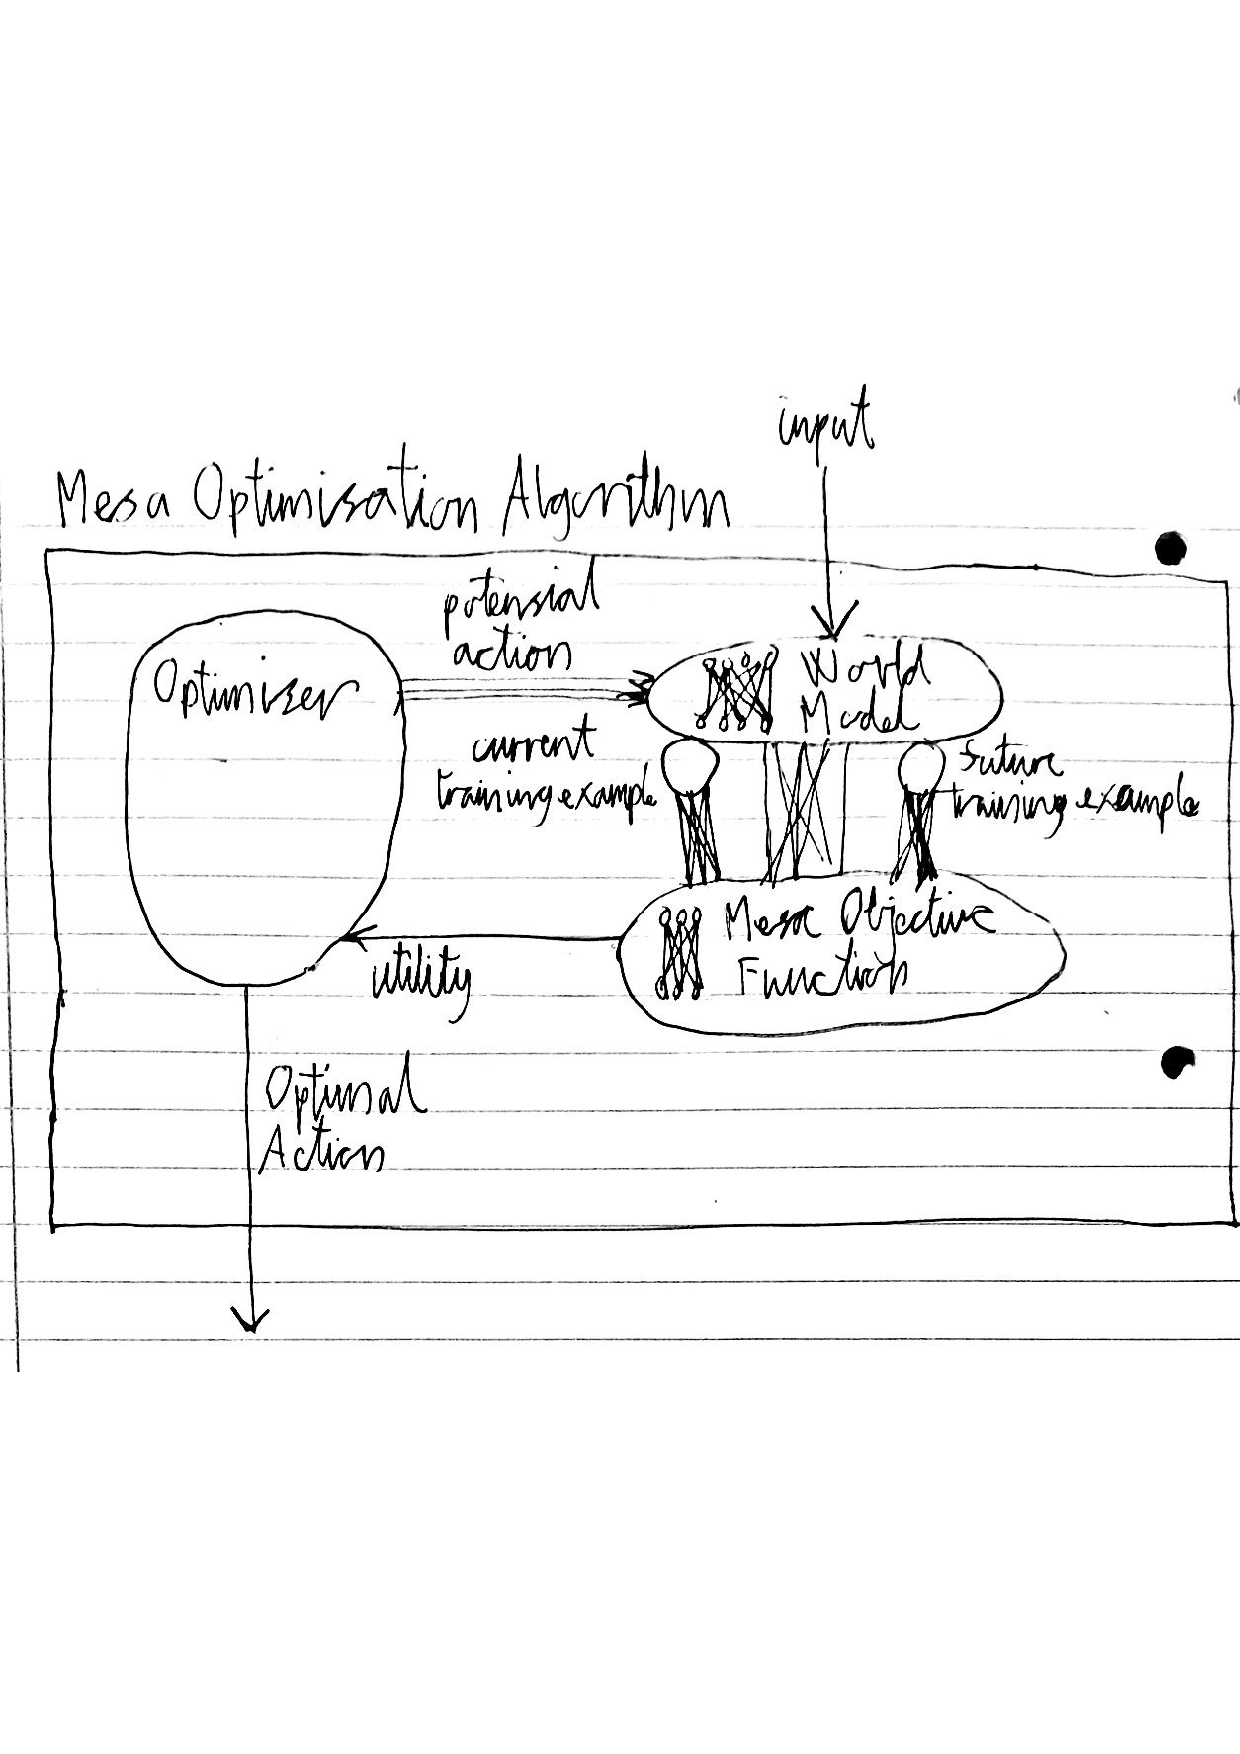
\includegraphics[width=\linewidth]{mesaoptdiagram}
        \caption{Diagram of a mesa optimiser}
        \label{fig:figure1}
    \end{figure}
\section{Related Works}\label{sec:relatedworks}

\section{Method}\label{sec:method}

\section{Experiments}\label{sec:experiments}

\section{Conclusion}\label{sec:conclusion}

\bibliography{timeinductivebias}
\bibliographystyle{plain}
\begin{appendix}
    \section*{Appendix}
\end{appendix}
\end{document}